\documentclass[a4paper]{article}
\usepackage[a4paper,margin=25mm]{geometry}
\usepackage{graphicx,subcaption}
\usepackage{amsmath,amsfonts}
\usepackage[ruled,vlined]{algorithm2e}
\usepackage{tikz}
\usepackage{accents}
\usepackage{cite}
\newcommand{\rvec}[1]{\accentset{\rightarrow}{#1}}
\title{Notes on Hierarchical Softmax}
\author{G.A. Jarrad}
\begin{document}
\maketitle
\numberwithin{equation}{section}
\numberwithin{figure}{section}
\numberwithin{table}{section}

\section{Introduction}

In the context of natural language processing, it is common to maintain a list ${\cal V}$ of vocabulary words, which is usually
extracted from one or more training corpora of text documents that have been suitably tokenised.
Typically, the frequency of each token is observed, and the top $V=|{\cal V}|$ most common tokens form the vocabulary.
The vocabulary ${\cal V}$ is typically ordered, either lexicographically or by descending frequency.

When it comes to representing a given word token, $w_i\in{\cal V}$, 
it can be uniquely indexed by its position $i$ in the ordered list.
Thus, for the example vocabulary ${\cal V} = \{{\tt cat},{\tt dog},{\tt frog},{\tt mouse}\}$,
we might choose $w_2=\texttt{dog}$ and $w_4=\texttt{mouse}$, etc.
Alternatively, one can form a {\em 1-of-$V$} or {\em one-hot} vector containing $V-1$ zeros and a single one in the $i$-th
element. 
For example, $\texttt{repr}(\texttt{cat})=(1,0,0,0)$ and $\texttt{repr}(\texttt{frog})=(0,0,1,0)$, etc.
This latter representation is of fixed length $V$ --- 
the question is, can we form a shorter, but still unique, vector representation?

The answer is, yes we can. To do so, we first need to hierarchically partition the vocabulary ${\cal V}$ into 
a binary tree representation, which we shall call ${\cal T}_{\cal V}$. 
One way to do this is to simply partition ${\cal V}$ into two roughly equally sized lists, and then
recursively partition each list until only single tokens remain in each innermost list.
Alternatively, we can utilise the word frequency $f_i$ of each token $w_i$ to produce the probability,
$p_i=f_i/\sum_{i'=1}^V f_{i'}$, that a word randomly sampled from the training corpora matches $w_i$.
Using these probabilities, one can then partition ${\cal V}$ into nested groups, e.g.\ according to
either Huffman or Fano coding (the latter method being simpler but producing less optimal code lengths).
Morin and Bengio\cite{Morin+Bengio-2005} indicate that the mean path length when taking word frequencies into account
is typically smaller than that for trees balanced equally across all words.
Alternatively, Mnih and Hinton~\cite{NIPS2008_3583} discuss some feature-driven algorithms for constructing
binary vocabulary trees.
Figure~\ref{fig:catdog} shows a simple (but unbalanced) binary tree representation of the example vocabulary. 
\begin{figure}[hbt]
\centering
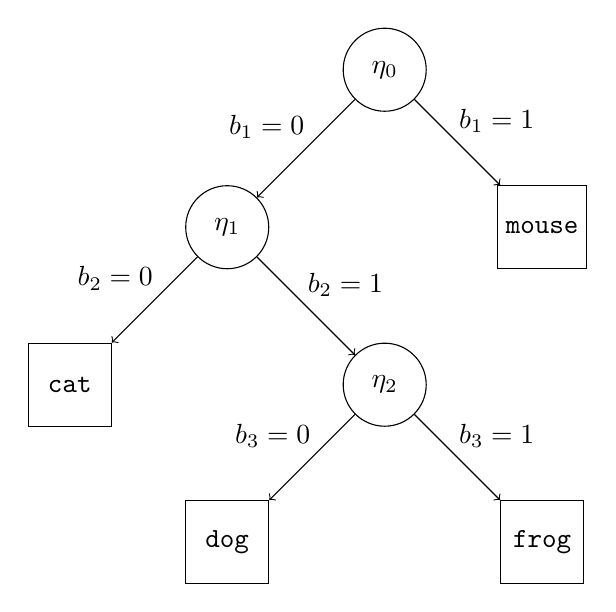
\begin{tikzpicture}[cnode/.style={draw,circle,minimum size=3em,inner sep=3pt}, rnode/.style={draw,rectangle,minimum size=3em,inner sep=3pt}]
    \node[cnode] (0) at (4,0) {$\eta_0$};
    \node[cnode] (1) at (2,-2) {$\eta_1$};
    \node[rnode] (2) at (6,-2) {\texttt{mouse}};
    \node[rnode] (3) at (0,-4) {\texttt{cat}};
    \node[cnode] (4) at (4,-4) {$\eta_2$};
    \node[rnode] (5) at (2,-6) {\texttt{dog}};
    \node[rnode] (6) at (6,-6) {\texttt{frog}};

    \draw[->] (0) edge node [pos=0.5, above] {\hspace*{-10mm}$b_1=0$} (1) ;
    \draw[->] (0) edge node [pos=0.5, above] {\hspace*{10mm}$b_1=1$} (2) ;
    \draw[->] (1) edge node [pos=0.5, above] {\hspace*{-10mm}$b_2=0$} (3) ;
    \draw[->] (1) edge node [pos=0.5, above] {\hspace*{10mm}$b_2=1$} (4) ;
    \draw[->] (4) edge node [pos=0.5, above] {\hspace*{-10mm}$b_3=0$} (5) ;
    \draw[->] (4) edge node [pos=0.5, above] {\hspace*{10mm}$b_3=1$} (6) ;
\end{tikzpicture}
\caption{\em An example of an unbalanced binary tree representation of a simple vocabulary.}
\label{fig:catdog}
\end{figure}

Note that the binary tree ${\cal T}_{\cal V}$ will contain $V$ leaf nodes, corresponding to the vocabulary words, and
$V-1$ internal nodes, corresponding to binary decision points. 
%We denote the set of leaf nodes by ${\cal N}_{\cal V}$,
%and the residual tree of purely internal nodes by ${\cal T}'_{\cal V}={\cal T}_{\cal V}\backslash {\cal N}_{\cal V}$.
Additionally, the tree will have a maximum of $L_{\cal V}$ levels, where
$L_{\cal V}\ge 1+\lceil\log_2 V\rceil$ (with equality holding if the tree is balanced).
Thus, any path $(\eta_{i_1},\eta_{i_2},\ldots,\eta_{i_n})$ 
from the root node $\eta_{i_1}\equiv\eta_{0}$ to a leaf node $\eta_{i_n}$ will pass through $n \le L_{\cal V}$ nodes.
This fact gives use scope for reducing the size of the unique word representation vectors.

It can be seen from Figure~\ref{fig:catdog} that each path through ${\cal T}_{\cal V}$ 
from the root node towards any leaf node
can be uniquely determined by specifying the 
sequence of binary branching decisions (0 for left, 1 for right) made along the path.
Thus, in this example we now have $\texttt{repr}(\texttt{cat})=(0,0)$, 
$\texttt{repr}(\texttt{dog})=(0,1,0)$, $\texttt{repr}(\texttt{frog})=(0,1,1)$
and $\texttt{repr}(\texttt{mouse})=(1)$.
These binary sequences collectively form the hierarchical representation of this vocabulary.
Note that, for our simple example, the maximum size of the representation vector is three, whereas it would be two for a balanced tree,
in contrast to the fixed size of four for the 1-of-$V$ representation.
In general, the size is reduced from $V$ to about $\log_2 V$ by the binary partitioning.

\section{Probability Model}

A typical natural language problem is to determine which word $w\in{\cal V}$ is appropriate in some context
\textbf{x}. In probabilistic terms, this amounts to computing $p(w\;|\;\textbf{x})\doteq p(\texttt{repr}(w)\;|\;\textbf{x})$.
Here we assume that we have some binary tree representation ${\cal T}_{\cal V}$ of the vocabulary ${\cal V}$,
such that $\texttt{repr}(w)=(b_1,b_2,\ldots,b_n)$.
In order to decompose this probabilistic model, first reconsider Figure~\ref{fig:catdog}.
Recalling that $\texttt{repr}(\texttt{frog})=(0,1,1)$, we see that
\begin{eqnarray}
p(\texttt{frog}\;|\;\textbf{x})
& = & p(b_1=0,b_2=1,b_3=1\;|\;\textbf{x})
\nonumber\\
& = & p(b_1=0\;|\;\textbf{x})\,p(b_2=1\;|\;\textbf{x},b_1=0)\,
p(b_3=1\;|\;\textbf{x},b_1=0,b_2=1)
\,.\nonumber
\end{eqnarray}
To make this more general, let $\rvec{\rho}_{1:j}=(b_1, b_2, \cdots, b_j)$ for $j=1,2,\ldots,n$,
where each binary decision $b_j$ takes its corresponding value from the $j$-th element of $\texttt{repr}(w)$.
Then we see that
\begin{eqnarray}
p(w\;|\;\textbf{x})
& = & \prod_{j=1}^n p(b_j\;|\;\textbf{x},\rvec{\rho}_{1:j-1})\,,
\label{eq:p:word}
\end{eqnarray}
where $\rvec{\rho}_{1:n}=\texttt{repr}(w)$, and $\rvec{\rho}_{1:0}=()$ by definition.

Notionally, each subpath, specified by $\rvec{\rho}_{1:j}$ for $j<n$,
terminates at some unique, internal node $\eta_k$ in ${\cal T}_{\cal V}$, indexed by
$k=\iota(\rvec{\rho}_{1:j})$. By definition, $\iota(())=0$, so that we always start from the root node $\eta_0$.
Consequently, we allow each internal node $\eta_k$ to have parameters ${\bf\theta}_k$.
Furthermore, we suppose that composing the context $\textbf{x}$ with node $\eta_k$
results in local features ${\bf\phi}_k({\bf x})={\bf\phi}({\bf x},{\bf\theta}_k)$.
Hence, each factor of equation~\eqref{eq:p:word} becomes
\begin{eqnarray}
p(b_j\;|\;\textbf{x},\rvec{\rho}_{1:j-1}) & \doteq &
p(b_j\;|\;{\bf\phi}_{k}({\bf x}),k=\iota(\rvec{\rho}_{1:j-1}))
\,,
\label{eq:p:word:term}
\end{eqnarray}
for $j=1,2,\ldots,n$ with $n=|\texttt{repr}(w)|$.

\subsection{Logistic Model}

In a neural network framework, the probability terms comprising equation~\eqref{eq:p:word} would represent an output layer
consisting of, for each internal node of the tree ${\cal T}_{\cal V}$, an activation function of an affine transformation of the input $\textbf{x}$.
Here we choose the logistic sigma activation function $\sigma(x)=1/(1+\exp{(-x)})$, and thus suppose that the local features of node $\eta_k$
are given by ${\bf\phi}_k({\bf x})=\alpha_k + {\bf \beta}_k^{T}{\bf x}$.
Hence, we take the probability of the $j$-th binary decision $b_j$ along a specified path $\rvec{\rho}_{1:n}$ to be
\begin{eqnarray}
p(b_j\;|\;{\bf x},\rvec{\rho}_{1:j-1}) & \doteq & \sigma((2b_j-1)(\alpha_k+{\bf \beta}_k^{T}{\bf x}))\,,
\end{eqnarray}
from equation~\eqref{eq:p:word:term}. We have made use of the fact that $1-\sigma(x)=\sigma(-x)$.

Note that the scalar output of the neural network for node $\eta_k$ must represent one of either $p(b_j=0\;|\;\cdots)$ or
$p(b_j=1\;|\;\cdots)$. It is common to choose the former; however, we choose the latter here, since during training of the neural network
one would optimise the parameters to minimise the `distance' between $p(b_j\;|\;\cdots)$ and the known value of $b_j$.
In other words, we desire $p(b_j=1\;|\;\cdots)\approx 1$ when $b_j=1$, and $p(b_j=1\;|\;\cdots)\approx 0$ when $b_j=0$.
Hence, each hierarchical vector representation exactly specifies the desired output probabilities.

\subsection{Optimal Path}

In order to find the (or a) word $w^*$ in the vocabulary that best matches the context ${\bf x}$, it would appear on the surface
that we need to evaluate $p(w\;|\;\textbf{x})$ for every $w\in{\cal V}$. However, we can do better. Note that:
\begin{itemize}
\item The probability factors $p(b_j\;|\;\textbf{x},\rvec{\rho}_{1:j-1})$ are available at every internal node of the binary tree ${\cal T}_{\cal V}$,
e.g.\ via one computational pass of the context ${\bf x}$ through a neural network;

\item The tree is in fact a directed acyclic graph, which allows us to apply a graph search algorithm.
\end{itemize}
Consequently, we can apply the $A^*$ search algorithm (albeit without a heuristic function).

To do so, we start with an empty {\em chart} (or {\em closed set}) ${\cal C}$ that will contain evaluated subpaths,
and an empty {\em priority queue} (or {\em open set}) ${\cal Q}$ that will contain subpaths to be evaluated.
We then insert the empty subpath $()$ onto ${\cal Q}$ with its default score.
Then repeatedly, while ${\cal Q}$ is not empty, we remove the best scoring subpath and: (i) if it terminates at a leaf node, return the word $w$;
or else (ii) insert the subpath into ${\cal C}$, evaluate the two binary decisions ($b=0$ and $b=1$), and insert each new subpath with its corresponding score onto ${\cal Q}$.
Pseudo-code for this method is given by Algorithm~\ref{alg:astar}.
Note that, based on the implementation, the chart ${\cal C}$ might or might not be required (depending upon whether or not it is used to reconstruct the optimal path via backtracking);
here we show a chartless version.
\begin{algorithm}[hbt]
 \SetAlgoLined
 \SetKwInOut{Input}{Input}\SetKwInOut{Output}{Output}
 \Input{Binary vocabulary tree ${\cal T}_{\cal V}$; word context ${\bf x}$}
 \Output{Word $w$; score $s$; path $\rho$}
 \BlankLine
 ${\cal Q}\leftarrow [\;]$\tcp*[r]{Initialise queue}
 $\eta\leftarrow\textbf{get\_root}({\cal T}_{\cal V})$\tcp*[r]{Obtain root node}
 $\nu\leftarrow\textbf{make\_node}(\texttt{node}=\eta, \texttt{path}=(),\texttt{score}=1)$\tcp*[r]{Construct score node}
 $Q\leftarrow\textbf{insert\_node}({\cal Q}, \nu)$\tcp*[r]{Insert score node}
 \While{$|{\cal Q}|>0$}{
  $({\cal Q}, \nu)\leftarrow\textbf{pop\_node}({\cal Q})$\tcp*[r]{Obtain highest-scoring node}
  $s\leftarrow\textbf{get\_value}(\nu, \texttt{score})$\tcp*[r]{Obtain score}
  $\rho\leftarrow\textbf{get\_value}(\nu, \texttt{path})$\tcp*[r]{Obtain path}
  $\eta\leftarrow\textbf{get\_value}(\nu, \texttt{node})$\tcp*{Obtain tree node}
  \eIf{$\textbf{is\_leaf}(\eta)$}{
   $w\leftarrow\textbf{get\_word}(\eta)$\tcp*[r]{Obtain word}
   \KwRet{$(w,s,\rho)$}\;
  }{
   $p\leftarrow\textbf{calc\_prob}(\eta, {\bf x})$\tcp*[r]{Compute probability of $b=1$}
   $s'\leftarrow[s(1-p),sp]$\tcp*[r]{Construct scores}
   \For{$b\in\{0,1\}$}{
    $\eta'\leftarrow\textbf{get\_child}(\eta, b)$\tcp*[r]{Obtain child node}
    $\rho'\leftarrow\rho\oplus(b)$\tcp*[r]{Construct child path}
    $\nu'\leftarrow\textbf{make\_node}(\texttt{node}=\eta', \texttt{path}=\rho', \texttt{score}=s'[b])$\tcp*[r]{Construct score node}
    $Q\leftarrow\textbf{insert\_node}({\cal Q}, \nu')$\tcp*[r]{Insert score node}
   }
  }
 }
 \caption{Find word with highest probability}
 \label{alg:astar}
\end{algorithm}

Note that this algorithm can easily be adapted to produce the top $N$ most probable words.
Also note that, in practice, it is better to sum (negative) log-probability scores rather than directly multiply probabilities,
otherwise for large vocabulary trees we run into the problem of underflow of vanishingly small probabilities.
There are in fact many more subtleties to implementing the $A^*$ algorithm, including: how to build the priority queue;
how to insert a node ranked by score;
where to insert a node into a batch of equally-scored nodes; etc. These issues will not be addressed here.

%%%%%%%%%%%%%%%%%%%%%%%%%%%%%%%%
\bibliography{hierarchical-softmax}{}
\bibliographystyle{plain}

\end{document}
